%!TEX root = SISC_elastic_3d.tex
\subsection{Semi-discretization of the elastic wave equation}\label{semi_discrete_form}

\begin{figure}[htbp]
	\centering
	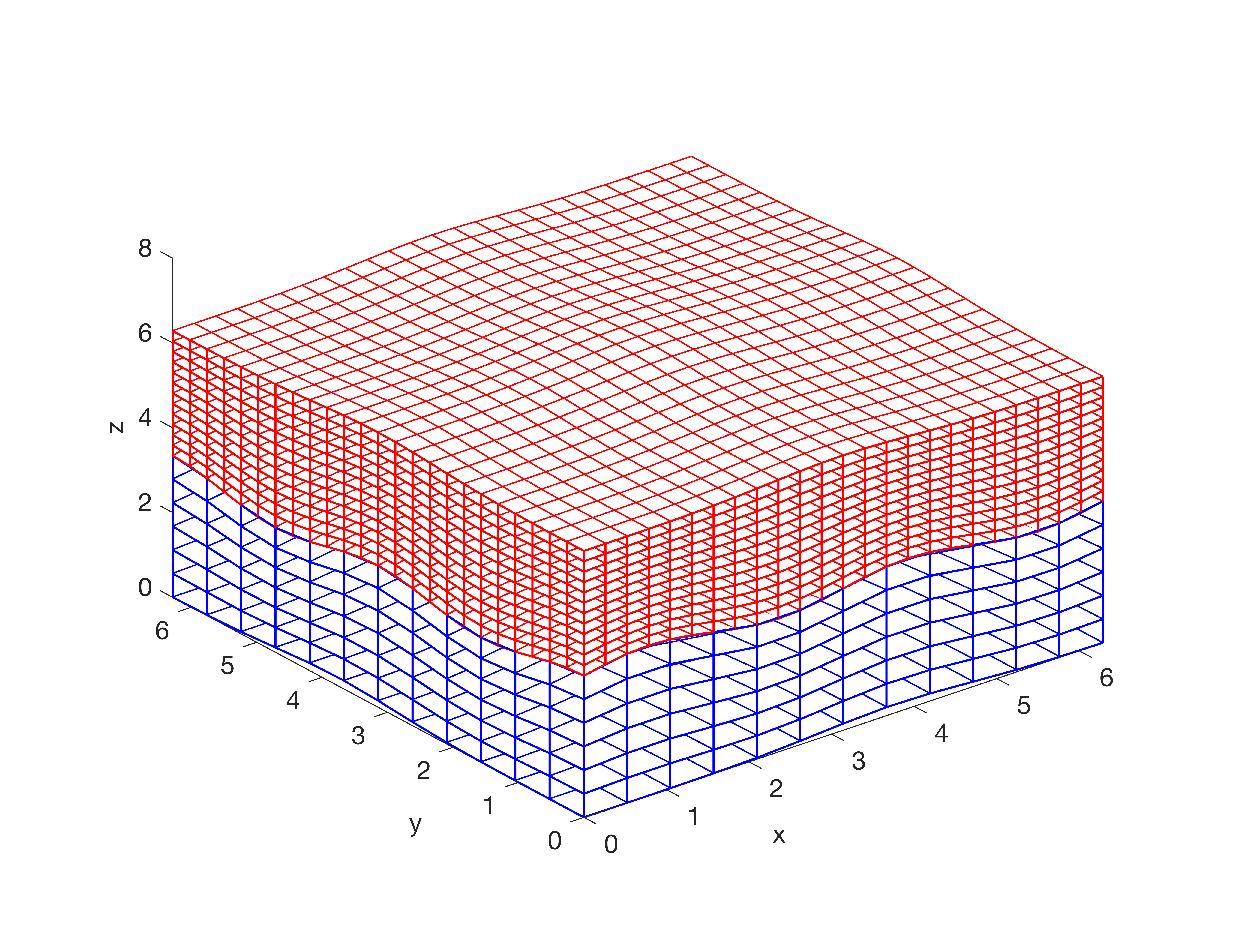
\includegraphics[width=0.6\textwidth,trim={0.4cm 0.7cm 0.8cm 1.4cm}, clip]{physical_discretization.eps}
	\caption{The sketch for the curvilinear mesh of the physical domain $\Omega$. The blue region is the spatial discretization of coarse subdomain $\Omega^c$ and the red region is the spatial discretization of the fine domain $\Omega^f$. Note that $x,y,z$ in the graph correspond to $x^{(1)}, x^{(2)}, x^{(3)}$ respectively. 
	 }\label{physical_discretization}
\end{figure}

In this section, we discretize the elastic wave equations (\ref{elastic_curvi}) and  (\ref{elastic_curvi_f}) with mesh refinement interface $\Gamma$. We assume the ratio of mesh sizes in the reference domains is $1:2$, that is the mesh sizes satisfy
\[h_1(n_1^h-1) = 1, \ \ \ h_2(n_2^h-1) = 1, \ \ \ h_3(n_3^h-1) = 1,\]
and
\[2h_1(n_1^{2h}-1) = 1, \ \ \ 2h_2(n_2^{2h}-1) = 1, \ \ \ 2h_3(n_3^{2h}-1) = 1,\]
respectively. Other ratios can be treated analogously. Figure \ref{physical_discretization} gives an illustration of the discretization of a physical domain. This is an ideal mesh if the wave speed in $\Omega^f$ is half of the wave speed in $\Omega^c$.

In seismic wave simulation, far-field boundary conditions are often imposed in the $x^{(1)}$ and $x^{(2)}$ directions. Here, our focus is on the numerical treatment of the interface conditions (\ref{interface_cond}). We assume periodic boundary conditions in $x^{(1)}$ and $x^{(2)}$, and ignore the boundaries in $x^{(3)}$. In Figure \ref{section_discretization}, we fix $x^{(2)} = 0$ and present the $x^{(1)}$-$x^{(3)}$ section of the domain $\Omega$ in both curvilinear space and parameter space.
\begin{figure}[htbp]
	\centering
	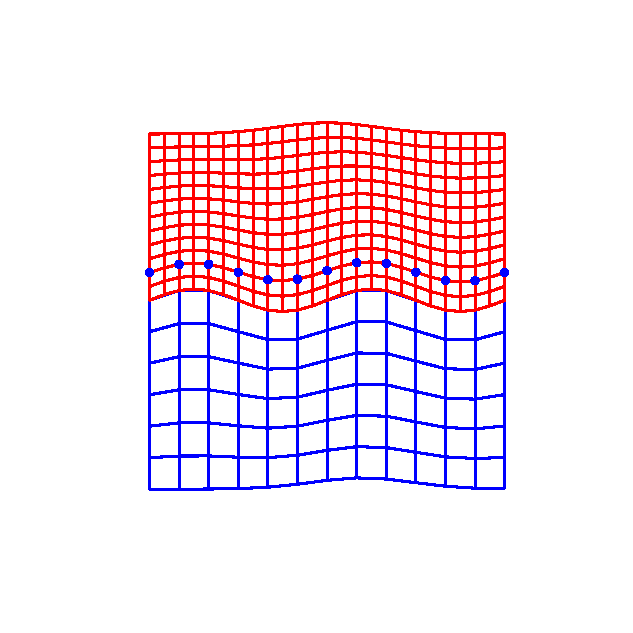
\includegraphics[width=0.45\textwidth,trim={1.0cm 2.0cm 1.0cm 1.8cm}, clip]{physical_section_discretization.eps}
	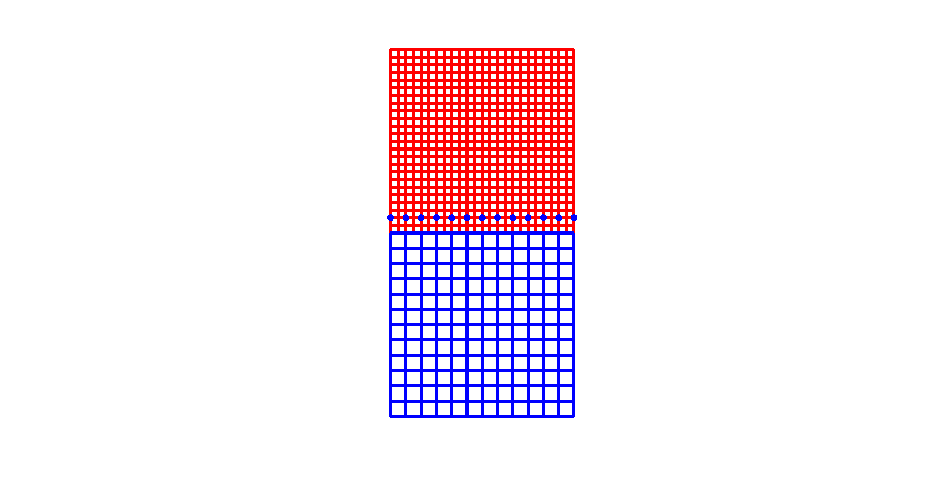
\includegraphics[width=0.45\textwidth,trim={1.0cm 2.0cm 1cm 1.8cm}, clip]{parameter_section_discretization.eps}
	\caption{The sketch of spatial discretization of $x^{(1)}$-$x^{(3)}$ section with $x^{(2)} = 0$. From the left to the right are for physical domain and parameter space, respectively. The blue dots are the ghost points for the coarse domain $\Omega^c$.}\label{section_discretization}
\end{figure}
 To condense notations, we introduce the multi-index notations
\[{\bf i} = (i,j,k),\ \ {\bf r}_{\bf i} = (r^{(1)}_i,r^{(2)}_j,r^{(3)}_k),\ \ {\bf x}_{\bf i} = (x^{(1)}_i,x^{(2)}_j,x^{(3)}_k),\]
then group different sets of grids as
\begin{equation*}
\begin{aligned}
	I_{\Omega^c} &= \{i = 1,2,\cdots,n_1^{2h}, j = 1,2,\cdots,n_2^{2h}, k = 1,2,\cdots,n_3^{2h}\},\\
	I_{\Gamma^c} & = \{i = 1,2,\cdots,n_1^{2h}, j = 1,2,\cdots,n_2^{2h}, k = n_3^{2h}\},\\
	I_{\Omega^f} &= \{i = 1,2,\cdots,n_1^h, j = 1,2,\cdots,n_2^h, k = 1,2,\cdots,n_3^h\},\\
	I_{\Gamma^f} & = \{i = 1,2,\cdots,n_1^{h}, j = 1,2,\cdots,n_2^{h}, k = 1\}.
\end{aligned}	
\end{equation*}
The physical coordinates of the coarse grid points and fine grid points follow from the mappings ${\bf x}_{\bf i} = {\bf X}^c({\bf r}_{\bf i})$ and ${\bf x}_{\bf i} = {\bf X}^f({\bf r}_{\bf i})$, respectively. We denote a grid function by
\[{\bf u}_{\bf i} = {\bf u}_{i,j,k} = {\bf u}({\bf x}_{\bf i}),\]
where ${\bf u}$ can be either a scalar or vector. 

In the spatial discretization, we only use ghost points in the coarse domain and do not use ghost points in the fine domain. Comparing with the approach of using ghost points in both domains, the system of linear equations at the interface becomes smaller and has a better structure. For the rest of the paper, the $\sim$ over an operator represents that the ghost points are used. Specifically, we approximate the elastic wave equation (\ref{elastic_curvi}) in $\Omega^c$ by
\begin{equation}\label{elastic_semi_c}
{\rho}_{\bf i}^{c}\frac{d^2{{\bf C}_{\bf i}}}{dt^2} = \frac{1}{J^c_{\bf i}}\wt{\mathcal{L}}^{2h} {{\bf C}}_{\bf i},\quad {\bf i}\in I_{\Omega^c},\quad t>0,
\end{equation}
where the discrete spatial operator is
\begin{equation}\label{L_operator}
\wt{\mathcal{L}}^{2h} {{\bf C}} = \left(\sum_{l=1}^2{Q}_l^{2h}({N}_{ll}^{2h}){\bf C}+\wt{{G}}_3^{2h}({N}_{33}^{2h}){{\bf C}}+\sum_{l=1}^3\sum_{m=1,m\neq l}^3{D}_l^{2h}({N}_{lm}^{2h}{D}_m^{2h}{\bf C})\right).
\end{equation}
Here, the components of the vector ${\bf C}$ are ${\bf C} = (C^{(1)}, C^{(2)}, C^{(3)})^T$. Note that we have used the same notation ${\bf C}$ in semi-discretization formula (\ref{L_operator}) and continuous formula (\ref{elastic_curvi}). But ${\bf C}$ represents a grid function when it is in a semi-discretization formula and a continuous function when it is in a continuous framework. The term $Q_l^{2h}(N_{ll}^{2h}){\bf C}$ approximates $\bar{\partial}_l(N_{ll}\bar{\partial}_l{\bf C})$ for $ l = 1,2$; $\wt{G}_3^{2h}(N_{33}^{2h}){\bf C}$ approximates $\bar{\partial}_3(N_{33}\bar{\partial}_3 {\bf C})$; and $D_{l}^{2h}(N_{lm}^{2h}D_m^{2h}{\bf C})$ approximates $\bar{\partial}_l(N_{lm}\bar{\partial}_m {\bf C})$ for  $l,m = 1,2,3, l\neq m$. The precise definitions of these terms are given in  Appendix \ref{appendix_cdomain}.

Next, we approximate the elastic wave equation (\ref{elastic_curvi_f}) on the fine grids. We first consider all fine grid points that are not located at the interface $\Gamma$. The semi-discretization  is
\begin{equation}\label{elastic_semi_f}
{\rho}_{\bf i}^{f}\frac{d^2{{\bf F}_{\bf i}}}{dt^2} = \frac{1}{J^f_{\bf i}}{\mathcal{L}}^{h} {{\bf F}}_{\bf i},\quad {\bf i}\in I_{\Omega^f}\backslash I_{{\Gamma^f}},\quad t>0.
\end{equation}
Here, the discrete spatial operator is
\begin{equation}\label{Lf_operator}
{\mathcal{L}}^{h} {{\bf F}} = \left(\sum_{l=1}^2{Q}_l^{h}({N}_{ll}^h){\bf F}+{G}_3^{h}({N}_{33}^h){\bf F}+\sum_{l=1}^3\sum_{m=1,m\neq l}^3{D}_l^{h}({N}_{lm}^{h}{D}_m^{h}{\bf F})\right),
\end{equation}
where the components of the vector ${\bf F}$ are ${\bf F} = (F^{(1)}, F^{(2)}, F^{(3)})^T$. Note that, like in the coarse domain, we also use the same notation ${\bf F}$ in semi-discretization formula (\ref{Lf_operator}) and continuous formula (\ref{elastic_curvi_f}). But ${\bf F}$ has different meanings when it is used in different framework as in the coarse domain. The terms $Q_l^{h}(N_{ll}^{h}){\bf F}, l = 1,2$ approximate $\bar{\partial}_l(N_{ll}\bar{\partial}_l{\bf F})$; ${G}_3^{h}(N_{33}^{h}){\bf F}$ approximates $\bar{\partial}_3(N_{33}\bar{\partial}_3 {\bf F})$; and $D_{l}^{h}(N_{lm}^{2h}D_m^{h}{\bf F}), l,m = 1,2,3, l\neq m$ approximate the terms $\bar{\partial}_l(N_{lm}\bar{\partial}_m {\bf F})$. Here, ${Q}_l^{h}({N}_{ll}^h){\bf F}, l = 1,2$ and ${D}_l^{h}({N}_{lm}^{h}{D}_m^{h}{\bf F})$ are defined similar as those in (\ref{L_operator}), but with the grids in $I_{\Omega^f}\backslash I_{{\Gamma^f}}$. The definition of ${{G}}_3^{h}({N}_{33}^{h}){\bf F}$ are shown in Appendix \ref{appendix_fdomain}.

For the approximation at the interface $\Gamma$, we obtain the numerical solution by injection using a scaled interpolation operator
\begin{equation}\label{continuous_sol}
{\bf F}_{\bf i} = {\mathcal{P}}{\bf C}_{{\bf i}'},\quad {\bf i}\in I_{\Gamma^f},\quad {{\bf i}'}\in I_{\Gamma^c}.
\end{equation}
It imposes the continuity of the solution at the interface $\Gamma$. 

For energy stability, the operator ${\mathcal{P}}$ must be in a specific form
\[{\mathcal{P}} = (\mathcal{J}^h_\Gamma \bm{\Lambda}^h)^{-\frac{1}{2}}({\bf P}\otimes{\bf I})(\mathcal{J}^{2h}_\Gamma \bm{\Lambda}^{2h})^{\frac{1}{2}}.\]
Here, ${\bf P}$ is a $n_1^hn_2^h\times n_1^{2h}n_2^{2h}$ interpolation matrix. Since the mesh refinement ratio is $1:2$, the stencils of the fourth order accurate interpolation operator ${\bf P}$ in two dimensions have four cases, see the illustration in  Figure \ref{interpolation}; and 
\[\mathcal{J}_{\Gamma}^h = J^{h}_{\Gamma} \otimes {\bf I},\quad {\bm{\Lambda}^h} = \Lambda^h\otimes {\bf I},\]
where both $J_{\Gamma}^h$ and $\Lambda^h$ are $n_1^{2h}n_2^{2h}\times n_1^{2h}n_2^{2h}$ diagonal matrices, the diagonal elements of $J_{\Gamma}^h$ and $\Lambda^{h}$ are $J^f$ and $|\nabla_x R^{f,(3)}|$ evaluated at fine grid points in $I_{\Gamma^f}$, respectively. ${\bf I}$ is $3\times 3$ identity matrix. As for $\mathcal{J}_{\Gamma}^{2h}$ and ${\bm{\Lambda}^{2h}}$, they have similar definitions with $\mathcal{J}_{\Gamma}^{h}$ and ${\bm{\Lambda}^{h}}$ but correspond to the coarse grid points in $I_{\Gamma^c}$.

We note that \eqref{continuous_sol} is equivalent to the more complicated form
\begin{equation}\label{elastic_semi_f_i}
{\rho}^f_{\bf i} \frac{d^2{\bf F}_{\bf i}}{dt^2} =
\frac{1}{J^f_{\bf i}}(\mathcal{L}^h{\bf F}_{\bf i} + {\bm \eta}_{\bf i}), \quad {\bf i}\in I_{\Gamma^f}
\end{equation}
with 
\begin{equation}\label{eta}
{\bm \eta}_{\bf i} = {\rho}^f_{\bf i}J^f_{\bf i}\wt{\mathcal{P}}\left(\frac{1}{\rho^c_{{\bf i}'}J^c_{{\bf i}'}}\wt{\mathcal{L}}^{2h} {\bf C}_{{\bf i}'}\right) - \mathcal{L}^{h}{\bf F}_{\bf i}, \quad {\bf i}\in I_{\Gamma^f},\quad {{\bf i}'}\in I_{\Gamma^c},
\end{equation}
which is useful in the energy analysis in the next section. The variable $\bm \eta$ in (\ref{eta}) is approximately zero with a second order truncation error, which is of the same order as the boundary stencil of the SBP operator. %Therefore, it does not affect the overall accuracy of the semi-discretization. 

For the simplicity of analysis, we introduce a general notation for the schemes (\ref{elastic_semi_f}) and (\ref{elastic_semi_f_i}) in the fine domain $\Omega^f$,
\begin{align}\label{fine_scheme}
{\rho}^f_{\bf i}\frac{d^2{\bf F}_{\bf i}}{dt^2} =\frac{1}{J^f_{\bf i}}\hat{\mathcal{L}}^h{\bf F}_{\bf i} = \left\{
\begin{aligned}
&\frac{1}{J^f_{\bf i}}(\mathcal{L}^h{\bf F}_{\bf i} +{\bm \eta}_{\bf i}), \quad {\bf i}\in I_{\Gamma^f}\\
&\frac{1}{J^f_{\bf i}}\mathcal{L}^h{\bf F}_{\bf i},\quad\quad\quad {\bf i}\in I_{\Omega^f}\backslash I_{\Gamma^f} 
\end{aligned}
\right. \quad t > 0.
\end{align}
In computer implementation, we use \eqref{continuous_sol} to obtain the solution on the interface of the fine domain. The reason for introducing    \eqref{elastic_semi_f_i} is that it will be helpful in the energy analysis in Sec.~\ref{sec_energy}.

The following condition imposes continuity of traction at the interface, the first equation in (\ref{interface_cond}),
\begin{equation}\label{continuous_traction}
(\Lambda^{c}_{{\bf i}'}J_{{\bf i}'}^{c})^{-1}\wt{\mathcal{A}}_3^{2h}{\bf C}_{{\bf i}'}
= {\mathcal{R}}\Big((\Lambda^f_{\bf i}{ J}^f_{\bf i})^{-1}(\mathcal{A}_3^h{\bf F}_{\bf i}-h_3\omega_1{\bm \eta}_{\bf i})\Big), \quad {\bf i}\in I_{\Gamma^f},\quad {{\bf i}'}\in I_{\Gamma^c}.
\end{equation}
The term $h_3\omega_1{\bm \eta}_{\bf i}$ in (\ref{continuous_traction}) originates from the fact that ghost points are only used in the coarse domain but not in the fine domain. The term is important for energy stability, as shown in Theorem \ref{thm1}. It is a penalty term on the order of the truncation error and thus (\ref{continuous_traction})  provides a valid way of enforcing the continuity of traction force at the interface.  In (\ref{continuous_traction}), $\omega_1$ is the first entry in the scalar product (\ref{inner_product}), $\Lambda_{{\bf i}'}^c$ and $\Lambda_{\bf i}^f$ store the values of functions $|\nabla_x R^{c,(3)}|$ and $|\nabla_x R^{f,(3)}|$ evaluated at the grid points in $I_{\Gamma^c}$ and $I_{\Gamma^f}$, respectively. We have used the notation
\begin{equation}\label{hatAf}
\mathcal{A}_3^h{\bf F} = {N}_{31}^{h}{D}^h_1{\bf F} + {N}_{32}^h{D}^h_2{\bf F} + {N}_{33}^h\mathcal{D}_3^h{\bf F},
\end{equation}
where ${N}_{3l}^hD_l^h{\bf F}, l = 1,2,3$ approximate $N_{3l}\bar{\partial}_l{\bf F}$ and are given in Appendix \ref{traction_f}; and the other notation 
\begin{equation}\label{hatAc}
\wt{\mathcal{A}}_3^{2h}{\bf C} = {N}_{31}^{2h}{D}^{2h}_1{\bf C} + {N}_{32}^{2h}{D}^{2h}_2{\bf C} + {N}_{33}^{2h}\wt{\mathcal{D}}^{2h}_3{\bf C}.
\end{equation}
Here, ${N}_{3l}^{2h}D_l^{2h}{\bf C}, l = 1,2$ approximate $N_{3l}\bar{\partial}_l{\bf C}$ and they have similar definitions as those in (\ref{hatAf}), but correspond to the grids in $I_{\Gamma^c}$; and ${N}_{33}^{2h}\wt{\mathcal{D}}^{2h}_3{\bf C}$ approximates $N_{33}\bar{\partial}_3{\bf C}$ are shown in Appendix \ref{traction_c}. The condition \eqref{continuous_traction} determines the ghost points values in the coarse domain. Finally, the scaled restriction operator ${\mathcal{R}} $ has the structure 
 \[{\mathcal{R}} =  (\mathcal{J}^{2h}_\Gamma \bm{\Lambda}^{2h})^{-\frac{1}{2}}({\bf R}\otimes{\bf I})(\mathcal{J}^{h}_\Gamma \bm{\Lambda}^h)^{\frac{1}{2}},\]
 where ${\bf I}$ is a $3\times3$ identity matrix, ${\bf R}$ is a $n_1^{2h}n_2^{2h}\times n_1^hn_2^h$ restriction operator in two dimensions which is determined by the compatibility condition ${\bf R}=\frac{1}{4}{\bf P}^T$ and its stencil is presented in Figure \ref{restriction}. As will be seen later, the compatibility condition, as well as the scaling of the interpolation and restrictions, are essential for energy stability \cite{Lundquist2018}.

\begin{figure}%[htbp]
	\centering
	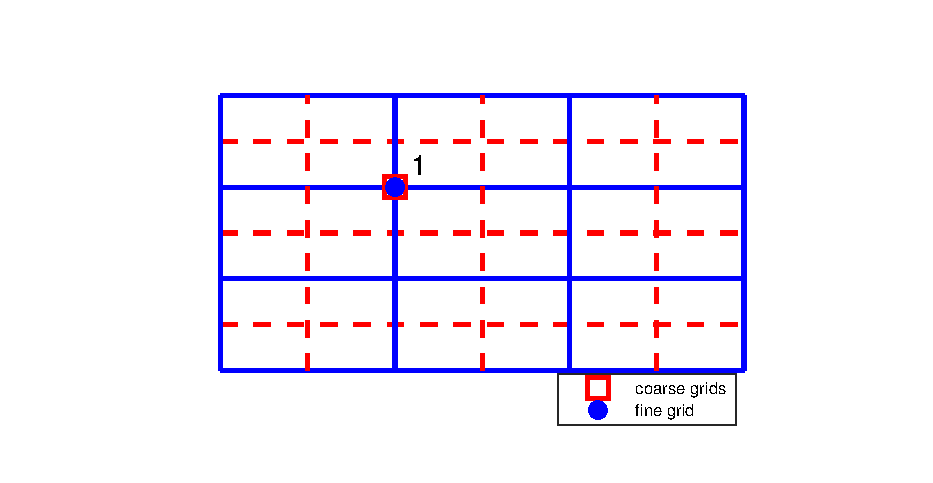
\includegraphics[width=0.24\textwidth,trim={1.8cm 0.8cm 1.4cm 1.2cm}, clip]{interpolation1.eps}
	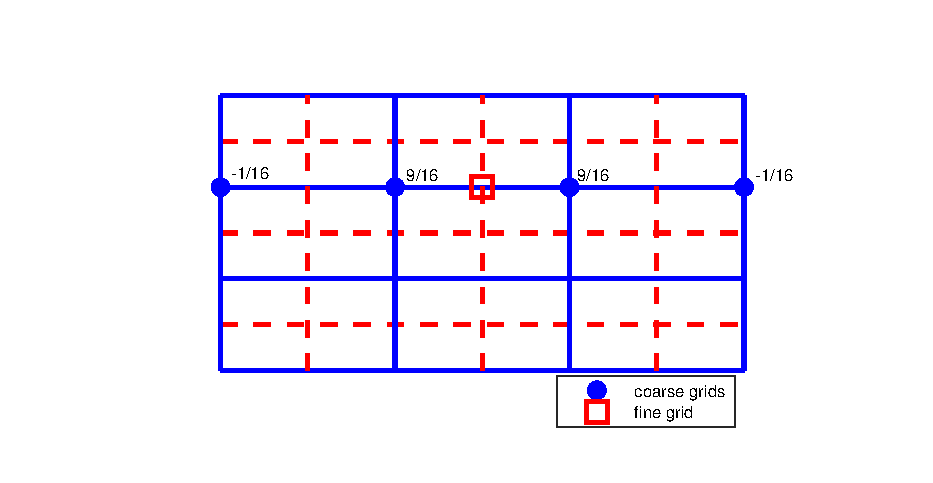
\includegraphics[width=0.24\textwidth,trim={1.8cm 0.8cm 1.4cm 1.2cm}, clip]{interpolation2.eps}
	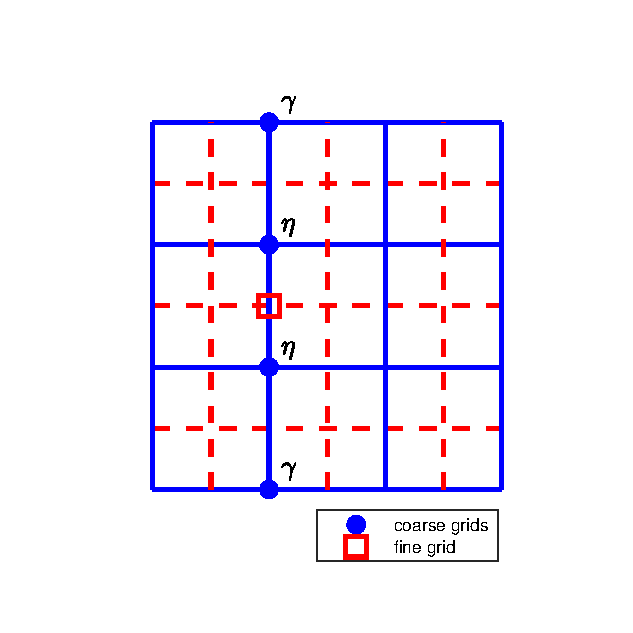
\includegraphics[width=0.24\textwidth,trim={1.8cm 0.8cm 1.4cm 1.2cm}, clip]{interpolation3.eps}
	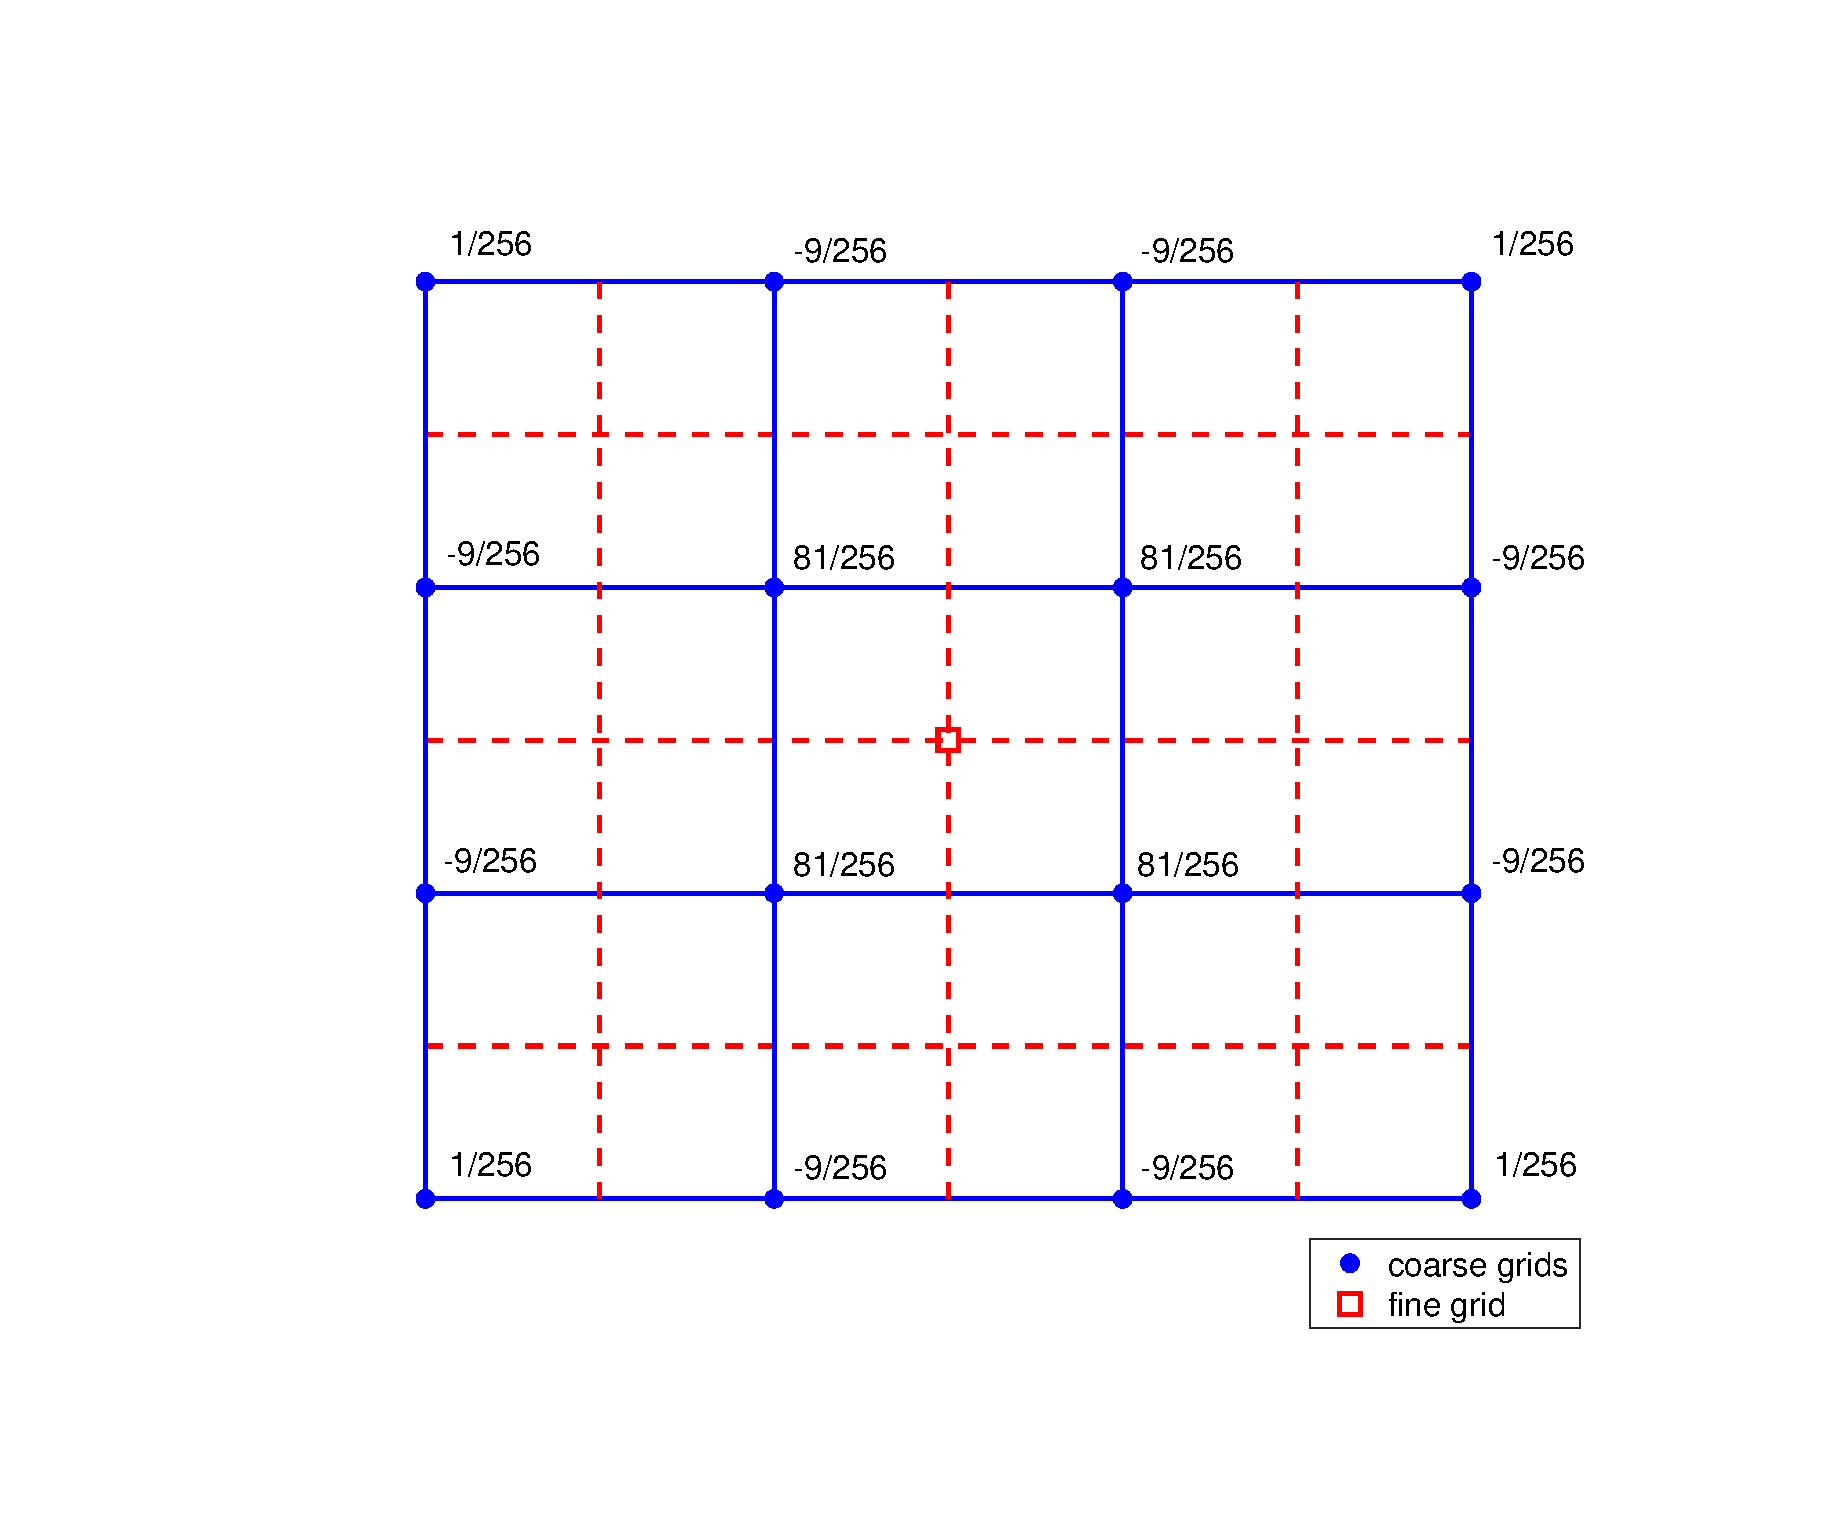
\includegraphics[width=0.24\textwidth,trim={1.8cm 0.8cm 1.4cm 1.2cm}, clip]{interpolation4.eps}
	\caption{The sketch for the stencils of fourth order interpolation operator ${\bf P}$ in two dimensions with parameters $\gamma = -\frac{1}{16}$, $\eta = \frac{9}{16}$, $\mu = 1$, $\alpha = \frac{1}{256}$, $\beta = -\frac{9}{256}$ and $\theta = \frac{81}{256}$. }\label{interpolation}
\end{figure}
\begin{figure}[htbp]
	\centering
	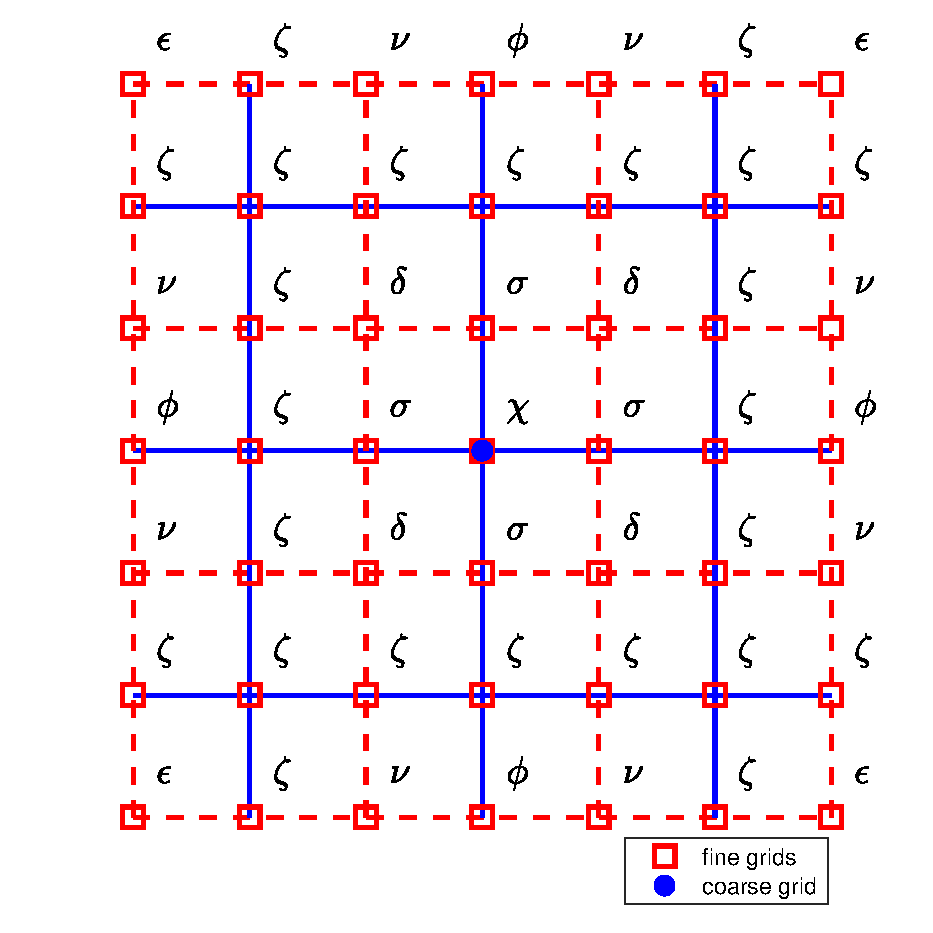
\includegraphics[width=0.6\textwidth]{restriction.eps}
	\caption{The sketch for the stencil of fourth order restriction operator ${\bf R}$ in two dimensions with parameters $\epsilon = \frac{1}{1024}$, $\nu = -\frac{9}{1024}$, $\phi = -\frac{16}{1024}$, $\delta = \frac{81}{1024}$, $\sigma = \frac{144}{1024}$, $\chi = \frac{256}{1024}$ and $\zeta = 0$.}\label{restriction}
\end{figure}




